% !TEX TS-program = pdflatex
% ROS2_ARCHITECTURE.tex
% ROS 2 software architecture for the autonomous TEC atmospheric-water
% PV-cleaning robot. Companion to prototype_design_report.tex (ch. 6-7:
% mechanics, control) and FIVE_DAY_WRAPUP_PLAN.tex (4-tile bench prototype).
% All plant numbers trace to output/tec_robot_results.json.
\documentclass[11pt,a4paper]{article}

\usepackage[margin=2.3cm]{geometry}
\usepackage[T1]{fontenc}
\usepackage{lmodern}
\usepackage{microtype}
\usepackage{amsmath,amssymb}
\usepackage{siunitx}
\sisetup{per-mode=symbol,range-phrase={--},range-units=single}
\usepackage{booktabs}
\usepackage{tabularx}
\usepackage{array}
\usepackage{caption}
\usepackage{enumitem}
\usepackage{listings}
\usepackage{xcolor}
\usepackage{tikz}
\usetikzlibrary{positioning}
\usepackage{cite}
\usepackage[hidelinks]{hyperref}
\usepackage{titlesec}
\titleformat{\section}{\large\bfseries}{\thesection.}{0.5em}{}
\titleformat{\subsection}{\normalsize\bfseries}{\thesubsection}{0.5em}{}
\emergencystretch=1.5em

% code style for URDF / YAML / launch listings
\lstset{
  basicstyle=\ttfamily\footnotesize,
  columns=fullflexible,
  keepspaces=true,
  breaklines=true,
  frame=single,
  framerule=0.3pt,
  xleftmargin=1em,
  showstringspaces=false,
}
% typewriter path names with line breaks allowed after underscores
\newcommand{\topic}[1]{{\ttfamily\def\_{\textunderscore\allowbreak}#1}}
\newcommand{\pkg}[1]{{\ttfamily\def\_{\textunderscore\allowbreak}#1}}
\newcolumntype{L}[1]{>{\raggedright\arraybackslash}p{#1}}

\title{\textbf{ROS~2 Software Architecture}\\[0.4em]
\large Autonomous Thermoelectric Atmospheric-Water PV-Cleaning Robot\\[0.2em]
\normalsize Two-tier design: ROS~2 on a Raspberry Pi~4 with micro-ROS on the ESP32}
% Plant: rail-guided carriage, rack-and-pinion fall-line drive (8 kg, 0.96 m brush).
\author{Rahma El-Hamouly, Graduation Project (REE598)}
\date{12 June 2026}

\begin{document}
\maketitle

\begin{abstract}
\noindent
This document specifies the ROS~2 software architecture for the \SI{8}{\kilo\gram}
rail-guided PV-cleaning robot designed in the prototype design report. The robot
rides guide rails on a panel tilted up to \ang{24} and a rack-and-pinion drive moves
it along the fall line; one full-width \SI{0.96}{\metre} brush cleans the panel in a
single down-and-up sweep (\SI{66.7}{\second} per panel) and consumes self-harvested
distilled water per event. The architecture has two tiers: a Raspberry Pi~4 runs
ROS~2 (motion, sweep coverage, mission supervision, logging) and an ESP32
runs micro-ROS plus bare-metal control loops (drive PWM, the \SI{10}{\hertz} TEC
cold-plate PID, safety reflexes). The document defines the package layout with a
URDF skeleton, the full node/topic/service/action interface with QoS classes and
rates, the micro-ROS serial budget (\SI{4.9}{\kilo B\per\second} of
\SI{11.5}{\kilo B\per\second} available at \num{115200}\,baud), the launch and
simulation plan, and the mapping onto the 4-tile bench prototype, which reuses the
AWG and logging packages without the drive stack.
\end{abstract}

{\setcounter{tocdepth}{1}\tableofcontents}
\newpage

% =============================================================================
\section{Scope}
% =============================================================================
The prototype design report fixed the plant: an \SI{8}{\kilo\gram} rail-guided
carriage with a full-width \SI{0.96}{\metre} brush, a 69-tile TEC1-12706 condenser array
(\SI{1.01}{\litre\per\day}, \SI{4.16}{\kilo\watt\hour\per\litre} thermoelectric),
and a supervisory state machine Idle\,$\to$\,Harvest\,$\to$\,Store\,$\to$\,Clean\,$\to$\,Dock
with a PID loop on the TEC cold-plate temperature. That control concept was written
for a single ESP32 with no middleware. This document ports it to ROS~2 so that the
REE599 experiments can be run, logged, and replayed with standard tooling, and so
that the navigation and coverage logic can be tested in simulation before the robot
touches a real panel. All plant constants used here trace to
\texttt{output/tec\_robot\_results.json}.

% =============================================================================
\section{Compute architecture}
% =============================================================================

\subsection{Why one MCU is not enough}
The ESP32 in the original design (240\,MHz dual-core, \SI{520}{\kilo B} SRAM, no MMU)
cannot host a ROS~2 stack: the rmw/rcl layers, a DDS implementation, the coverage
action server, TF, and rosbag2 each assume a POSIX operating system and tens to
hundreds of megabytes of memory. Conversely, a Linux single-board computer is a poor
home for the hard-real-time loops: scheduling jitter on a non-RT kernel is of order
milliseconds, which is acceptable for a \SI{10}{\hertz} thermal loop in principle but
not for motor PWM, encoder capture, or the end-of-travel reversal reflex, where a
missed deadline on a \ang{24} slope lets the carriage overrun the rail end. The
standard resolution is a two-tier split \cite{belsare2023microros}: a Raspberry Pi~4
(\SI{4}{\giga B}, Ubuntu~24.04, ROS~2 Jazzy; everything below also builds on Humble)
runs the soft-real-time graph, and the ESP32 keeps the hard-real-time I/O under
micro-ROS, talking to the Pi over a UART at \num{115200}\,baud through the XRCE-DDS
agent. Figure~\ref{fig:tiers} shows the split; Table~\ref{tab:division} lists the
assignment rule applied to every function.

\begin{figure}[htb]
\centering
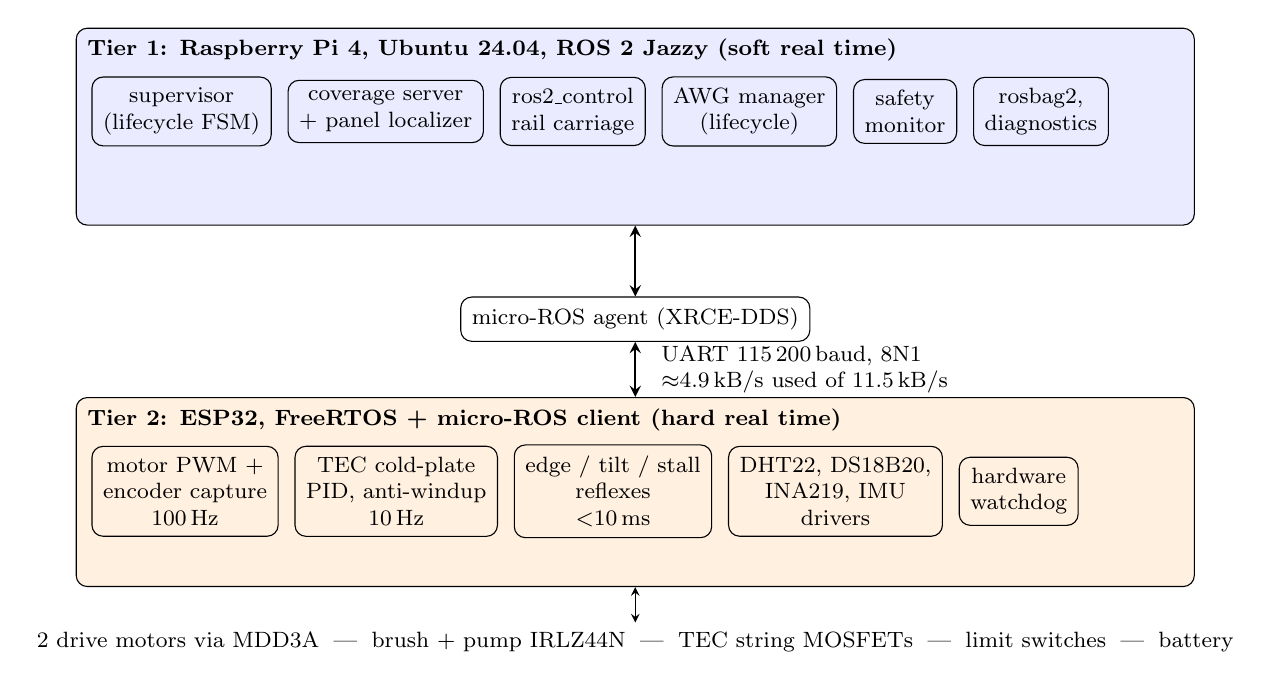
\begin{tikzpicture}[
  font=\footnotesize,
  box/.style={draw, rounded corners, align=center, inner sep=4pt},
  tier/.style={draw, rounded corners, inner sep=8pt},
  >=stealth]
% Pi tier
\node[box, fill=blue!8, minimum width=14.2cm, minimum height=2.5cm] (pi) {};
\node[anchor=north west, inner sep=4pt] at (pi.north west)
  {\textbf{Tier 1: Raspberry Pi 4, Ubuntu 24.04, ROS 2 Jazzy (soft real time)}};
\node[box, below=0.62cm of pi.north west, anchor=north west, xshift=2mm] (sup) {supervisor\\(lifecycle FSM)};
\node[box, right=2mm of sup] (nav) {coverage server\\+ panel localizer};
\node[box, right=2mm of nav] (base) {ros2\_control\\rail carriage};
\node[box, right=2mm of base] (awg) {AWG manager\\(lifecycle)};
\node[box, right=2mm of awg] (saf) {safety\\monitor};
\node[box, right=2mm of saf] (bag) {rosbag2,\\diagnostics};
% agent
\node[box, below=0.9cm of pi, minimum width=4.2cm] (agent) {micro-ROS agent (XRCE-DDS)};
% ESP32 tier
\node[box, fill=orange!12, below=0.7cm of agent, minimum width=14.2cm, minimum height=2.4cm] (esp) {};
\node[anchor=north west, inner sep=4pt] at (esp.north west)
  {\textbf{Tier 2: ESP32, FreeRTOS + micro-ROS client (hard real time)}};
\node[box, below=0.62cm of esp.north west, anchor=north west, xshift=2mm] (pwm) {motor PWM +\\encoder capture\\\SI{100}{\hertz}};
\node[box, right=2mm of pwm] (pid) {TEC cold-plate\\PID, anti-windup\\\SI{10}{\hertz}};
\node[box, right=2mm of pid] (rfx) {edge / tilt / stall\\reflexes\\$<$\SI{10}{\milli\second}};
\node[box, right=2mm of rfx] (sens) {DHT22, DS18B20,\\INA219, IMU\\drivers};
\node[box, right=2mm of sens] (wdt) {hardware\\watchdog};
\draw[<->, thick] (pi) -- (agent);
\draw[<->, thick] (agent) -- (esp)
  node[midway, right=2mm, align=left] {UART \num{115200}\,baud, 8N1\\$\approx$\SI{4.9}{\kilo B\per\second} used of \SI{11.5}{\kilo B\per\second}};
% hardware line
\node[below=0.45cm of esp, align=center] (hw)
  {2 drive motors via MDD3A \;|\; brush + pump IRLZ44N \;|\; TEC string MOSFETs \;|\; limit switches \;|\; battery};
\draw[<->] (esp) -- (hw);
\end{tikzpicture}
\caption{Two-tier compute architecture. The Pi owns everything that benefits from
ROS~2 tooling; the ESP32 owns everything with a hard deadline. Only compact custom
messages cross the serial bridge (Section~\ref{sec:bridge}).}
\label{fig:tiers}
\end{figure}

\begin{table}[htb]
\centering\small
\caption{Division of labour between the two tiers.}
\label{tab:division}
\begin{tabularx}{\textwidth}{@{}L{4.6cm}L{2.2cm}X@{}}
\toprule
\textbf{Function} & \textbf{Tier} & \textbf{Reason} \\
\midrule
Drive PWM to the MDD3A, drive-axis velocity PI, quadrature encoder capture (\SI{100}{\hertz}) & ESP32 & Deadline \SI{<1}{\milli\second} jitter; quadrature decode needs interrupts/timers; the MDD3A takes one PWM and one direction line per channel. \\
TEC cold-plate PID with anti-windup at $I_{max}=\SI{6}{\ampere}$ (\SI{10}{\hertz}) & ESP32 & Must survive Pi reboot; runs all night while the Pi is power-gated. \\
End-of-travel reversal, IMU tilt/fall trip, stall cutout, watchdog & ESP32 & Reflexes; must act in \SI{<10}{\milli\second} with no serial link in the loop. \\
Odometry integration, TF, EKF/complementary fusion & Pi & Floating-point heavy, no hard deadline, needed by TF consumers. \\
Fall-line sweep coverage action server & Pi & Plans and monitors the down-and-up sweep; \SI{20}{\hertz} is sufficient. \\
Mission FSM (Idle $\to$ Harvest $\to$ Store $\to$ Clean $\to$ Dock) & Pi (mirrored on ESP32) & Lifecycle node for introspection; ESP32 keeps a minimal Harvest/Store copy for power-gated nights. \\
Logging (rosbag2), diagnostics, parameter management & Pi & Thesis experiment data; needs storage and a filesystem. \\
\bottomrule
\end{tabularx}
\end{table}

\subsection{Why ROS 2}
Four features pay for the added mass of a middleware on a robot this small
\cite{macenski2022ros2}:
\begin{enumerate}[nosep]
\item \emph{Managed lifecycle nodes.} The AWG manager and the supervisor expose the
  standard configure/activate/deactivate transitions, so the bench prototype, the
  simulator, and the full robot can bring the same code up and down in a controlled
  order, and a fault can demote a node without killing the process.
\item \emph{ros2\_control and the nav2 ecosystem.} The single-axis carriage
  position/velocity control, odometry, and command limiting come from the maintained
  ros2\_control controllers rather than project code, and the coverage server can
  later be swapped for the nav2 complete-coverage server (for a future free-roaming
  variant) without touching the rest of the graph \cite{macenski2020marathon}.
\item \emph{Introspection.} \texttt{ros2 topic hz}, \texttt{ros2 doctor}, and the TF
  tree make integration faults visible in minutes. On the original bare-ESP32 design
  every debugging question required new firmware.
\item \emph{rosbag2.} Every thesis experiment (coverage accuracy, water-per-event,
  PID step response) becomes a bag file that can be replayed and re-analysed after
  the hardware is disassembled. This matters for a one-student project on a
  five-day build window.
\end{enumerate}

\subsection{Power note}
The energy budget in the design report allocates \SI{36}{\watt\hour\per\day} to the
MCU. A Pi~4 idles near \SI{2.7}{\watt}, so keeping it awake through a \SI{12}{\hour}
harvest night would add roughly \SI{32}{\watt\hour\per\day} and double that line
item. The architecture therefore power-gates the Pi outside Clean/Dock missions: the
ESP32 firmware retains a minimal local copy of the Harvest and Store states plus all
safety reflexes, and a GPIO from the ESP32 switches the Pi's \SI{5}{\volt} rail when
a cleaning mission or a logging session is due. During bench testing the Pi stays
powered, since logging is the point of the bench.

% =============================================================================
\section{Package layout}
% =============================================================================
Eight packages, one repository. Table~\ref{tab:packages} lists them;
all interface types live in \pkg{pvbot\_msgs} so the firmware and the Pi build from
one definition.

\begin{table}[htb]
\centering\small
\caption{Package layout.}
\label{tab:packages}
\begin{tabularx}{\textwidth}{@{}L{3.4cm}X@{}}
\toprule
\textbf{Package} & \textbf{Contents} \\
\midrule
\pkg{pvbot\_msgs} & Custom messages, services, actions: \texttt{WheelTicks}, \texttt{ImuRaw}, \texttt{AwgState}, \texttt{SafetyStatus}, \texttt{srv/SetSetpoint}, \texttt{action/CoverPanel}. Shared by firmware and Pi. \\
\pkg{pvbot\_description} & URDF/xacro of the chassis (Listing~\ref{lst:urdf}), meshes, \pkg{robot\_state\_publisher} launch. \\
\pkg{pvbot\_base} & \pkg{ros2\_control} hardware interface that maps drive commands and tick states onto the bridge topics; single-axis carriage controller and \pkg{joint\_state\_broadcaster} configuration (Listing~\ref{lst:yaml}). \\
\pkg{pvbot\_awg} & AWG manager lifecycle node: relays \topic{/awg/state}, owns the set-point and harvest start/stop services, tracks tank level against the \SI{0.6}{\litre} cleaning threshold. \\
\pkg{pvbot\_cleaning} & Brush and pump actuation services; interlocks pump against tank level and brush against motion state. \\
\pkg{pvbot\_navigation} & Panel localizer (odometry + IMU + end-of-travel re-registration) and the fall-line sweep coverage action server. \\
\pkg{pvbot\_safety} & Safety monitor: heartbeat watchdog on the bridge, tilt/battery limits, latched \topic{/safety/estop}, reset service. \\
\pkg{pvbot\_supervisor} & Mission FSM as a managed lifecycle node (Section~\ref{sec:supervisor}). \\
\pkg{pvbot\_bringup} & Launch trees (robot, simulation, bench), parameter files, rosbag2 profiles. \\
\bottomrule
\end{tabularx}
\end{table}

The firmware lives outside the ROS workspace as a PlatformIO project
(\pkg{pvbot\_firmware}) that vendors the micro-ROS client library and the
\pkg{pvbot\_msgs} type support.

\subsection{URDF skeleton}
Listing~\ref{lst:urdf} is the load-bearing subset of
\pkg{pvbot\_description/urdf/pvbot.urdf.xacro}: an \SI{8}{\kilo\gram} box carriage
(\qtyproduct{1.00 x 0.30 x 0.12}{\metre}, spanning the panel width), a prismatic
drive joint that moves the carriage along the rail fall line through a
\SI{30}{\milli\metre} pinion meshing a rack, the IMU frame, and the full-width
\SI{0.96}{\metre} brush as a continuous joint so its drag torque can be modelled in
simulation.

\begin{lstlisting}[language=XML, caption={URDF skeleton (inertias from the box and
cylinder formulas, rounded). The carriage rides the rail through a single prismatic
drive joint; the rack frame is fixed (world) so the joint coordinate is the
along-rail position.}, label={lst:urdf}]
<robot name="pvbot" xmlns:xacro="http://www.ros.org/wiki/xacro">
  <link name="rail_link"/>     <!-- fixed rail frame, panel fall line = +x -->

  <link name="base_link">
    <inertial>
      <mass value="8.0"/>  <!-- carriage + TEC tiles + tank (mean fill) -->
      <inertia ixx="0.0696" iyy="0.6763" izz="0.7273"
               ixy="0" ixz="0" iyz="0"/>
    </inertial>
    <collision><geometry><box size="1.00 0.30 0.12"/></geometry></collision>
  </link>

  <!-- rack-and-pinion drive modelled as one prismatic joint along the rail -->
  <joint name="carriage_joint" type="prismatic">
    <parent link="rail_link"/> <child link="base_link"/>
    <origin xyz="0 0 0" rpy="0 0 0"/>
    <axis xyz="1 0 0"/>                 <!-- fall line -->
    <limit lower="0.0" upper="2.0" effort="30.0" velocity="0.10"/>
  </joint>

  <link name="imu_link"/>      <!-- 0.0 0.0 0.06, identity rpy -->
  <link name="brush_link"/>    <!-- cylinder r=0.025 l=0.96, full width -->
  <joint name="brush_joint" type="continuous">
    <parent link="base_link"/> <child link="brush_link"/>
    <origin xyz="0.40 0 -0.05" rpy="-1.5708 0 0"/>
    <axis xyz="0 0 1"/>
  </joint>

  <ros2_control name="pvbot_hw" type="system">
    <hardware>
      <plugin>pvbot_base/BridgeSystem</plugin>  <!-- micro-ROS topics -->
    </hardware>
    <joint name="carriage_joint">
      <command_interface name="velocity"/>
      <state_interface name="position"/> <state_interface name="velocity"/>
    </joint>
  </ros2_control>
</robot>
\end{lstlisting}

\begin{lstlisting}[caption={Single-axis carriage controller parameters (excerpt of
\pkg{pvbot\_base/config/controllers.yaml}). The drive is a rack-and-pinion on one
joint, so the controller commands along-rail velocity directly.}, label={lst:yaml}]
carriage_controller:        # velocity controller on carriage_joint
  ros__parameters:
    joint: carriage_joint
    pinion_radius: 0.015     # m (30 mm pinion)
    publish_rate: 50.0       # /odom and TF, Hz
    max_velocity: 0.10       # m/s (cleaning sweep 0.06)
    cmd_timeout: 0.5         # s; stop if coverage server dies
\end{lstlisting}

With a geared encoder count of about \num{1000} ticks per pinion revolution the
odometric resolution is $2\pi r_p/1000 = \SI{0.094}{\milli\metre}$ per tick, far
below the control needs; on a positively meshed rack the drive does not slip, so
odometry is limited only by quantisation and rack pitch tolerance.

On the hardware side the \pkg{BridgeSystem} interface maps the single
\texttt{carriage\_joint} velocity command onto both \num{1}:\num{71} GA25-370
gearmotors through one Cytron MDD3A dual driver: the firmware sends one PWM and
one direction line per channel and reads the two quadrature encoders, averaging
their counts into the along-rail position. Because the two rails are mechanically
locked through the carriage, the two channels carry the same command. The MDD3A
brake mode doubles as the unpowered hold on the \ang{24} slope: when the
supervisor parks the carriage, the firmware drives both channels into brake
rather than coasting, so the carriage does not creep down the rail. The brush and
the pump are not on the driver at all; each is a single IRLZ44N low-side MOSFET
switched from an ESP32 pin, since neither load reverses, which is why the
actuator command in Table~\ref{tab:nodes} is an event-rate on/off rather than a
velocity stream.

% =============================================================================
\section{Nodes, topics, services, actions}
% =============================================================================
Table~\ref{tab:qos} defines four QoS classes; Table~\ref{tab:nodes} lists every
node with its interfaces. Sensor streams use best-effort delivery because a stale
sample is worse than a dropped one; commands and latched states use reliable
delivery. The e-stop and the supervisor state are transient-local so that a node
joining late (or restarting) immediately sees the current value.

\begin{table}[htb]
\centering\small
\caption{QoS classes used in Table~\ref{tab:nodes}.}
\label{tab:qos}
\begin{tabular}{@{}llll@{}}
\toprule
\textbf{Class} & \textbf{Reliability} & \textbf{Durability} & \textbf{History} \\
\midrule
S (sensor)    & best effort & volatile        & keep last 5 \\
C (command)   & reliable    & volatile        & keep last 1 \\
L (latched)   & reliable    & transient local & keep last 1 \\
D (diagnostic)& reliable    & volatile        & keep last 10 \\
\bottomrule
\end{tabular}
\end{table}

\begin{table}[p]
\centering\footnotesize
\caption{Node interface table. Arrows: $\uparrow$ published, $\downarrow$
subscribed. Types are standard unless prefixed \texttt{pvbot\_msgs}.}
\label{tab:nodes}
\begin{tabularx}{\textwidth}{@{}L{2.9cm}XL{0.8cm}L{1.5cm}@{}}
\toprule
\textbf{Node (package)} & \textbf{Interface} & \textbf{QoS} & \textbf{Rate} \\
\midrule
firmware bridge (ESP32, micro-ROS)
 & $\uparrow$ \topic{/bridge/wheel\_ticks} (\texttt{WheelTicks}) & S & \SI{50}{\hertz} \\
 & $\uparrow$ \topic{/bridge/imu\_raw} (\texttt{ImuRaw}) & S & \SI{50}{\hertz} \\
 & $\uparrow$ \topic{/bridge/awg\_state} (\texttt{AwgState}) & S & \SI{1}{\hertz} \\
 & $\uparrow$ \topic{/bridge/safety} (\texttt{SafetyStatus}) & S & \SI{10}{\hertz} \\
 & $\downarrow$ \topic{/bridge/wheel\_cmd} (\texttt{WheelCmd}) & C & \SI{20}{\hertz} \\
 & $\downarrow$ \topic{/bridge/actuator\_cmd} (\texttt{ActuatorCmd}) & C & event \\
 & serves \topic{/awg/set\_setpoint} (\texttt{srv/SetSetpoint}) & C & event \\
\midrule
\pkg{ros2\_control} + carriage controller (\pkg{pvbot\_base})
 & $\downarrow$ \topic{/cmd\_vel} (\texttt{Twist}, \texttt{linear.x} only) & C & \SI{20}{\hertz} \\
 & $\uparrow$ \topic{/odom} (\texttt{Odometry}), TF \texttt{odom$\to$base\_link} & S & \SI{50}{\hertz} \\
 & $\uparrow$ \topic{/joint\_states} (\texttt{JointState}) & S & \SI{50}{\hertz} \\
\midrule
\pkg{imu\_filter\_madgwick}
 & $\downarrow$ \topic{/bridge/imu\_raw}; $\uparrow$ \topic{/imu/data} (\texttt{Imu}) & S & \SI{50}{\hertz} \\
\midrule
panel localizer (\pkg{pvbot\_navigation})
 & $\downarrow$ \topic{/odom}, \topic{/imu/data}, \topic{/bridge/safety} & S & \SI{50}{\hertz} \\
 & $\uparrow$ \topic{/panel\_pose} (\texttt{PoseStamped}, panel frame) & S & \SI{50}{\hertz} \\
\midrule
coverage server (\pkg{pvbot\_navigation})
 & serves \topic{/cover\_panel} (\texttt{action/CoverPanel}) & C & --- \\
 & $\downarrow$ \topic{/panel\_pose}; $\uparrow$ \topic{/cmd\_vel} & S/C & \SI{20}{\hertz} \\
 & feedback: pass index, fraction complete & C & \SI{1}{\hertz} \\
\midrule
AWG manager (\pkg{pvbot\_awg}, lifecycle)
 & $\downarrow$ \topic{/bridge/awg\_state}; $\uparrow$ \topic{/awg/state} (relabelled) & S & \SI{1}{\hertz} \\
 & $\uparrow$ \topic{/awg/tank\_level} (\texttt{Float32}, litres) & L & on change \\
 & serves \topic{/awg/start\_harvest}, \topic{/awg/stop} (\texttt{Trigger}) & C & event \\
 & forwards \topic{/awg/set\_setpoint} to firmware & C & event \\
\midrule
cleaning node (\pkg{pvbot\_cleaning})
 & serves \topic{/cleaning/set\_brush}, \topic{/cleaning/set\_pump} (\texttt{SetBool}) & C & event \\
 & $\uparrow$ \topic{/bridge/actuator\_cmd} & C & event \\
\midrule
safety monitor (\pkg{pvbot\_safety})
 & $\downarrow$ \topic{/bridge/safety}, \topic{/imu/data}, \topic{/awg/state} & S & \SI{10}{\hertz} \\
 & $\uparrow$ \topic{/safety/estop} (\texttt{Bool}, latched) & L & on change \\
 & serves \topic{/safety/reset} (\texttt{Trigger}) & C & event \\
\midrule
supervisor (\pkg{pvbot\_supervisor}, lifecycle)
 & $\downarrow$ \topic{/awg/tank\_level}, \topic{/safety/estop}, \topic{/awg/state} & L/S & --- \\
 & action client of \topic{/cover\_panel}; service client of AWG and cleaning & C & event \\
 & $\uparrow$ \topic{/supervisor/state} (\texttt{String}) & L & on change \\
\midrule
\pkg{diagnostic\_aggregator}
 & $\downarrow$ \topic{/diagnostics}; $\uparrow$ \topic{/diagnostics\_agg} & D & \SI{1}{\hertz} \\
\midrule
\pkg{rosbag2} (record)
 & $\downarrow$ experiment topic set (Table~\ref{tab:bag}) & --- & --- \\
\bottomrule
\end{tabularx}
\end{table}

% =============================================================================
\section{micro-ROS bridge and serial budget}
\label{sec:bridge}
% =============================================================================
The bridge carries only the six \texttt{pvbot\_msgs} types in
Table~\ref{tab:budget}. Everything else is derived on the Pi. The compact types
exist because the standard messages do not fit the link:
\texttt{sensor\_msgs/Imu} serialises to roughly \SI{300}{B} (orientation,
covariances, header with string frame id), so publishing it at \SI{50}{\hertz}
would need about \SI{15}{\kilo B\per\second}, more than the entire link.
\texttt{nav\_msgs/Odometry} is around \SI{720}{B}; integrating odometry on the Pi
from \SI{12}{B} tick messages avoids that cost and keeps the firmware free of
floating-point pose mathematics.

At \num{115200}\,baud, 8N1 framing yields \num{11520}\,B/s. XRCE-DDS adds about
\SI{20}{B} per message (session header, stream and sequence fields, framing and
CRC) \cite{belsare2023microros}. Table~\ref{tab:budget} sums payload and overhead:
\SI{4.9}{\kilo B\per\second}, a utilisation of \SI{43}{\percent}, leaving headroom
of a factor 2.3 for retransmissions and parameter traffic. If later sensors exceed
the budget, the ESP32's WiFi UDP transport raises the ceiling by two orders of
magnitude; the bench prototype already uses it (Section~\ref{sec:bench}).

\begin{table}[htb]
\centering\small
\caption{Serial budget at \num{115200}\,baud (\num{11520}\,B/s effective).
Payload sizes are CDR-aligned; overhead is \SI{20}{B} per message.}
\label{tab:budget}
\begin{tabular}{@{}llS[table-format=2.0]S[table-format=2.0]S[table-format=4.0]@{}}
\toprule
\textbf{Topic} & \textbf{Direction} & {\textbf{Payload (B)}} & {\textbf{Rate (Hz)}} & {\textbf{B/s incl.\ overhead}} \\
\midrule
\topic{wheel\_ticks}  & MCU $\to$ Pi & 12 & 50 & 1600 \\
\topic{imu\_raw}      & MCU $\to$ Pi & 28 & 50 & 2400 \\
\topic{safety}        & MCU $\to$ Pi & 8  & 10 & 280 \\
\topic{awg\_state}    & MCU $\to$ Pi & 40 & 1  & 60 \\
\topic{wheel\_cmd}    & Pi $\to$ MCU & 8  & 20 & 560 \\
\topic{actuator\_cmd} & Pi $\to$ MCU & 4  & 1  & 24 \\
\midrule
\textbf{Total} & & & & 4924 \\
\bottomrule
\end{tabular}
\end{table}

\paragraph{What never crosses the bridge.}
The drive velocity PI loop, the \SI{10}{\hertz} TEC cold-plate PID with its
anti-windup clamp at \SI{6}{\ampere}, the end-of-travel reversal interrupt, the IMU
tilt/fall trip, the motor stall cutout (\SI{>200}{\milli\second} overcurrent), and
the hardware watchdog all close locally on the ESP32. The design rule: any loop
whose failure can damage the robot or drop it off the panel must not depend on the
serial link, the agent process, or the Pi being awake. The Pi-side safety monitor
adds a second, slower layer (Section~\ref{sec:safety}); losing the bridge degrades
the system to the firmware's safe behaviour (stop motors, hold TEC mode, raise the
local fault flag), which is the same state the robot wakes up in.

% =============================================================================
\section{Coverage and localization without SLAM}
% =============================================================================
The workspace is a single known rectangle, about \qtyproduct{1.0 x 2.0}{\metre}. The
carriage spans the panel width on the guide rails, so coverage is one-dimensional:
the full-width \SI{0.96}{\metre} brush clears the whole width in a single fall-line
sweep, and the only path variable is the along-rail position. SLAM brings nothing
here: the glass surface is featureless and reflective (hostile to both lidar and
visual odometry), the map is known a priori, and the sweep is a single
down-and-up traverse of about \SI{4}{\metre}. The localizer dead-reckons the
along-rail coordinate in a fixed panel frame and re-registers at each rail end.

There is no cross-track coverage error to control. Because the rack-and-pinion drive
is positively meshed it does not slip, so the along-rail odometry error is set by
encoder quantisation and rack pitch tolerance rather than wheel slip, and the
end-of-travel switches reset it once per stroke. Two effects still matter, and the
design pins them down rather than mapping:

\begin{enumerate}[nosep]
\item \emph{End-of-travel re-registration.} Each half of the sweep ends on a limit
  switch closure at a known rail end, which resets the along-rail coordinate exactly.
  Error accumulates over one \SI{2}{\metre} stroke, not over the whole mission.
\item \emph{Gravity-referenced alignment.} On a plane tilted \ang{24} the gravity
  vector measured by the accelerometer fixes the carriage attitude relative to the
  fall line, so the localizer has an absolute pitch/roll reference of a few degrees
  without magnetometer or gyro integration drift, which confirms the carriage is
  square to the rails through the stroke.
\item \emph{Trivial decomposition.} A full-width sweep on an obstacle-free panel
  needs no cell decomposition \cite{choset2000coverage}; the ``planner'' is a
  parameterised stroke generator: one down-and-up traverse, about \SI{4}{\metre}
  total, \SI{66.7}{\second} at \SI{0.06}{\metre\per\second}.
\end{enumerate}

The coverage server is a plain action server (\texttt{action/CoverPanel}: goal =
panel length and sweep speed; feedback = stroke phase and fraction complete;
result = covered area estimate and water used). A nav2 plugin was considered and
rejected for the robot's first iteration: the nav2 stack assumes a costmap, a
global planner, and a controller server, all of which would be configured to do
nothing on a single rail with one degree of freedom. The action interface is
deliberately identical in shape to the nav2 coverage server's, so the swap remains
a one-launch-file change if a later free-roaming variant (a rooftop unit that
traverses between panel rows) needs real planning \cite{macenski2020marathon}.

% =============================================================================
\section{Supervisor: lifecycle FSM, not a behaviour tree}
\label{sec:supervisor}
% =============================================================================
The supervisor is a managed lifecycle node wrapping a table-driven finite-state
machine, the direct port of the ESP32 supervisor from the design report.
Table~\ref{tab:fsm} gives the transition table.

A behaviour tree was the alternative \cite{colledanchise2018bt}. The FSM wins for
this robot on three grounds. The mission is a fixed cycle with five states and no
runtime re-composition; the BT's strength, reactive subtree reuse, has nothing to
operate on. The transition table below is the same artifact that was already
verified for the bare-ESP32 design and that the firmware's minimal night-time
supervisor must mirror; keeping both sides as the same FSM makes the equivalence
checkable by inspection. And the thesis must argue safety: enumerating five states
and nine guarded transitions is a complete argument, while a BT requires reasoning
about tick order and halting semantics. The lifecycle wrapper adds what a raw FSM
lacks: the supervisor itself can be configured, activated, and deactivated by the
launch system and by the safety monitor, and its state is visible to standard
tooling.

\begin{table}[htb]
\centering\small
\caption{Supervisor transition table. Guards are evaluated on the topics of
Table~\ref{tab:nodes}; RTC = real-time clock, SoC = battery state of charge.}
\label{tab:fsm}
\begin{tabularx}{\textwidth}{@{}lllX@{}}
\toprule
\textbf{From} & \textbf{To} & \textbf{Trigger} & \textbf{Guard} \\
\midrule
Idle    & Harvest & RTC night window & dew margin $\ge\SI{5}{\kelvin}$ feasible (Mode A), SoC above reserve \\
Harvest & Store   & RTC day or margin lost & condensate present \\
Store   & Idle    & transfer complete & --- \\
Idle    & Clean   & soiling schedule due & \topic{/awg/tank\_level} $\ge\SI{0.6}{\litre}$, no e-stop, daylight \\
Clean   & Dock    & \topic{/cover\_panel} result received & --- \\
Clean   & Dock    & \topic{/cover\_panel} aborted & always (water remaining logged) \\
Dock    & Idle    & charge complete & SoC threshold \\
any     & Safe    & \topic{/safety/estop} latched & always; motors stopped, pump off \\
Safe    & Idle    & \topic{/safety/reset} called & operator only \\
\bottomrule
\end{tabularx}
\end{table}

% =============================================================================
\section{Safety layers}
\label{sec:safety}
% =============================================================================
Safety is split by latency, not by importance. The ESP32 reflex layer
(\SI{<10}{\milli\second}: end-of-travel reversal, tilt/fall trip at the IMU interrupt,
stall cutout, hardware watchdog on the \SIrange{10}{50}{\milli\second} control
loop) acts without consulting the Pi and reports after the fact through
\topic{/bridge/safety}. The Pi-side safety monitor handles everything slower: it
watches the \SI{10}{\hertz} firmware heartbeat and latches \topic{/safety/estop}
if three periods are missed (\SI{300}{\milli\second} detection), enforces battery
and temperature envelopes, and deactivates the supervisor through its lifecycle
interface rather than killing processes, so the FSM lands in the Safe state with
its context intact. \topic{/safety/estop} is transient-local: any node that
restarts learns the latched state before it can act. The carriage controller's
\SI{0.5}{\second} \texttt{cmd\_vel} timeout (Listing~\ref{lst:yaml}) is the final
backstop if the coverage server itself dies mid-pass: the controller stops the
drive, and the ESP32 brakes both channels.

% =============================================================================
\section{Launch and simulation plan}
% =============================================================================

\subsection{Launch tree}
\begin{lstlisting}[caption={Bringup launch tree. Each leaf is independently
testable; the bench omits the left branch entirely.}, label={lst:launch}]
pvbot_bringup/launch/
  robot.launch.py                  # full robot
    description.launch.py         # robot_state_publisher (URDF)
    base.launch.py                # ros2_control + controllers
    micro_ros_agent.launch.py     # serial /dev/ttyUSB0 115200
    navigation.launch.py          # panel localizer + coverage server
    awg.launch.py                 # AWG manager (lifecycle)
    cleaning.launch.py
    safety.launch.py
    supervisor.launch.py          # lifecycle FSM
    diagnostics.launch.py
    record.launch.py              # optional, arg record:=true
  sim.launch.py                   # Gazebo harness (below)
  bench.launch.py                 # 4-tile bench (Section 10)
\end{lstlisting}

\subsection{Gazebo harness}
The simulation world is one tilted panel: a \qtyproduct{1.0 x 2.0}{\metre} plane at
\ang{24} with glass-like friction coefficients, plus the URDF of
Listing~\ref{lst:urdf} driven by \pkg{gz\_ros2\_control} in place of the bridge
hardware interface. Contact sensors on the panel border emulate the limit
switches and publish the same \texttt{SafetyStatus} bits as the firmware, so the
localizer and coverage server run unmodified. A mock AWG node publishes synthetic
\topic{/awg/state} and ramps \topic{/awg/tank\_level}, letting the full
Idle$\to$Clean$\to$Dock cycle run in simulation. Three experiments run in the
harness before hardware: coverage completeness versus injected odometry noise
(\SIrange{1}{3}{\percent} systematic), edge re-registration behaviour with
simulated switch hysteresis, and supervisor fault injection (kill the coverage
action mid-pass, drop the mock bridge, force the e-stop).

\subsection{Bag recording for thesis experiments}
Table~\ref{tab:bag} estimates the recording load. A full \SI{66.7}{\second}
cleaning sweep is about \SI{5}{MB} uncompressed and around \SI{1.5}{MB} with the
zstd-compressed writer, so a complete day of trials fits in well under
\SI{100}{MB} on the Pi's SD card. Bags are the primary thesis artifacts: coverage
accuracy comes from \topic{/panel\_pose} replay, water-per-event from
\topic{/awg/tank\_level} deltas, and the PID step response from
\topic{/awg/state} during set-point changes.

\begin{table}[htb]
\centering\small
\caption{rosbag2 budget for one \SI{66.7}{\second} cleaning sweep.}
\label{tab:bag}
\begin{tabular}{@{}lS[table-format=2.0]S[table-format=3.0]S[table-format=2.1]@{}}
\toprule
\textbf{Topic} & {\textbf{Rate (Hz)}} & {\textbf{Msg size (B)}} & {\textbf{kB/s}} \\
\midrule
\topic{/odom}          & 50 & 720 & 36.0 \\
\topic{/imu/data}      & 50 & 300 & 15.0 \\
\topic{/tf}            & 50 & 250 & 12.5 \\
\topic{/joint\_states} & 50 & 150 & 7.5 \\
\topic{/panel\_pose}   & 50 &  90 & 4.5 \\
others (\topic{/awg/state}, \topic{/diagnostics\_agg}, feedback) & {---} & {---} & 1.5 \\
\midrule
\textbf{Total} & & & 77.0 \\
\bottomrule
\end{tabular}
\end{table}

% =============================================================================
\section{Mapping to the 4-tile bench prototype}
\label{sec:bench}
% =============================================================================
The bench prototype (4 TEC tiles, expected yield about \SI{59}{\gram\per\day}, no chassis)
exercises the AWG half of the architecture with the same packages and a different
launch file. \texttt{bench.launch.py} starts the micro-ROS agent on the WiFi UDP
transport (the bench ESP32 sits in a humidified enclosure away from the logging
laptop, and serial tethering is inconvenient there), the AWG manager, diagnostics,
and rosbag2; the drive, navigation, cleaning, safety-motion, and supervisor nodes
never start. Table~\ref{tab:bench} gives the mapping. The firmware image is the
same binary with the motor and switch drivers compiled out; the
\topic{/bridge/awg\_state} stream, the set-point service, and the \SI{10}{\hertz}
PID are byte-identical to the robot's. A \SI{12}{\hour} overnight bench log at
\SI{1}{\hertz} telemetry is roughly \SI{25}{MB} uncompressed, so storage is not a
constraint. The point of running the bench under ROS~2 rather than a serial
logger: the PID step-response and condensation-onset experiments produce the same
bag format as the robot experiments, and every analysis script written for the
bench transfers to the full system.

\begin{table}[htb]
\centering\small
\caption{Package subset on the 4-tile bench.}
\label{tab:bench}
\begin{tabular}{@{}lll@{}}
\toprule
\textbf{Package} & \textbf{Robot} & \textbf{Bench} \\
\midrule
\pkg{pvbot\_msgs}        & yes & yes \\
\pkg{pvbot\_awg}         & yes & yes \\
\pkg{pvbot\_bringup}     & \texttt{robot.launch.py} & \texttt{bench.launch.py} \\
micro-ROS transport      & UART \num{115200} & WiFi UDP \\
\pkg{pvbot\_description} & yes & no \\
\pkg{pvbot\_base}        & yes & no \\
\pkg{pvbot\_navigation}  & yes & no \\
\pkg{pvbot\_cleaning}    & yes & no \\
\pkg{pvbot\_safety}      & yes & heartbeat + thermal limits only \\
\pkg{pvbot\_supervisor}  & yes & no (manual service calls) \\
\bottomrule
\end{tabular}
\end{table}

% =============================================================================
\section{Summary of design decisions}
% =============================================================================
Two tiers, with the boundary drawn at hard real time: ROS~2 Jazzy on a power-gated
Raspberry Pi~4, micro-ROS on the ESP32, six compact message types on a
\num{115200}\,baud UART running at \SI{43}{\percent} utilisation. No SLAM: a
rail-guided carriage dead-reckons the single along-rail coordinate in a fixed panel
frame, bounded per stroke by end-of-travel re-registration and a gravity-referenced
attitude reference on the \ang{24} slope. Coverage is one full-width fall-line sweep,
served by a plain action server shaped like the nav2 interface so it can be replaced
when a free-roaming variant needs real planning. The mission supervisor stays a finite-state machine, now wrapped in
a lifecycle node, because it must remain provably equivalent to the minimal
copy that keeps harvesting on the ESP32 while the Pi sleeps. The 4-tile bench runs
the identical AWG package over WiFi UDP, so bench data and robot data share one
format from the first experiment onward.

\bibliographystyle{IEEEtran}
\bibliography{references}

\end{document}
